%%********************************************************************
%% Technische Hochschule Ingolstadt 
%%
%% To be used as style template for seminar papers in the 
%% Master's Programme AI Engineering of Autonomous Systems
%% Faculty of Electrical Engineering and Information Technology
%%
%% by Prof. Dr.-Ing. Michael Mecking  
%% based on a style file by Prof. Dr.-Ing. Munir Georges
%%********************************************************************

\documentclass[11pt, titlepage, english, a4paper]{article}

\usepackage[top=1.2in, bottom=1.4in, inner=1.1in, outer=1.1in]{geometry}

\usepackage[utf8]{inputenc}
\usepackage[english]{babel}         %% an English document with English setting and hyphanation
\usepackage{algorithmic}            %% number of commands for typesetting popular algorithmic constructs
\usepackage{listings}               %% typeset programs (programming code) within LaTeX
\usepackage{longtable}              %% write tables that continue to the next page
\usepackage{float}                  %% prevents repositioning of tables using [H]
\usepackage{fancyhdr,lipsum}        %% control of headers and footers 
\usepackage{lmodern}                %% modern font family 
\usepackage[T1]{fontenc}            %% 8-bit font encoding... more glyphs... easier copy&paste from the output (pdf) files

\usepackage{amsmath,bm}             %% ams math symbols
\usepackage{amsbsy}                 %% bold mathematics symbols where appropriate fonts exist
\usepackage{amsfonts}
\usepackage{amssymb}
\usepackage{eulervm}                %% Don Knuth's beautiful (my favourite!) math font
\usepackage{fixmath}                %% uppercase Greek be typeset in italic style

\usepackage[pdftex]{graphicx}
\usepackage[pdftex]{xcolor}
\usepackage[autostyle]{csquotes}    %% quotation according to language requirements
\usepackage{units}
\usepackage{hhline}
\usepackage{titling}
\usepackage{blindtext}
\usepackage{multirow}
\usepackage{lastpage}
\usepackage{afterpage}
\usepackage{hyperref}               %% hypertext in LaTeX

%%%%%%%%%%%%%%%%%%%%%%%%%%%%%%%%%%%%%%%%%%%%%%%%%%%%%%%%%%
%%  TikZ setup
\usepackage{tikz}                   %% add more libraries if needed
\usetikzlibrary{arrows,automata,shadows,positioning,decorations.pathreplacing,matrix,calc,%
backgrounds,patterns,shapes,shapes.gates.logic.IEC,intersections,through}

%%%%%%%%%%%%%%%%%%%%%%%%%%%%%%%%%%%%%%%%%%%%%%%%%%%%%%%%%%
%%  Definition of mathematical functions/operators for simpler syntax
\DeclareMathOperator{\sign}{sign}
\DeclareMathOperator{\Mod}{mod}
\DeclareMathOperator{\artanh}{artanh}
\DeclareMathOperator{\arcosh}{arcosh}
\DeclareMathOperator{\arc}{arc}
\DeclareMathOperator{\Arg}{Arg}
\renewcommand{\Re}{\mathrm{Re}}
\renewcommand{\Im}{\mathrm{Im}}
\DeclareMathOperator{\spn}{span}
\DeclareMathOperator{\defekt}{def}
\DeclareMathOperator{\diag}{diag}
\DeclareMathOperator{\grad}{grad}
\DeclareMathOperator{\argmin}{arg\,min}
\DeclareMathOperator{\argmax}{arg\,max}

%%%%%%%%%%%%%%%%%%%%%%%%%%%%%%%%%%%%%%%%%%%%%%%%%%%%%%%%%% 
%%  use the provided LaTeX-style file for your seminar paper
%%********************************************************************
%% Technische Hochschule Ingolstadt 
%%
%% author: Prof. Dr.-Ing. Michael Mecking  
%% based on Prof. Dr.-Ing. Munir Georges' 2021 style file.
%%
%% To be used as style template for seminar papers in the 
%% E-faculty Master's Programme 
%% AI Engineering of Autonomous Systems
%%********************************************************************

\fancyhf{}

\renewcommand{\headrulewidth}{0.1pt}
%\fancyhead[RO]{\nouppercase{\rightmark}}
\fancyhead[RO]{\includegraphics[width=0.5cm]{thi_logo_b_RGB.png} }
\raggedbottom
\fancypagestyle{plain}{%
    \fancyhf{}%
    \renewcommand{\headrulewidth}{0pt}%
    \fancyhf[lef,rof]{\thepage}%
}

\makeatletter
\def\cleardoublepage{\clearpage\if@twoside \ifodd\c@page\else
	\hbox{}
	\vspace*{\fill}
	\begin{center}
	\end{center}
	\vspace{\fill}
	\thispagestyle{empty}
	\newpage
	\if@twocolumn\hbox{}\newpage\fi\fi\fi}
\makeatother

\clearpage{\pagestyle{empty}\cleardoublepage}
\pagestyle{fancy}
\setlength{\headheight}{25pt}
\renewcommand{\sectionmark}[1]{\markright{\thesection.\ #1}}

\linespread{1.3}

\makeatletter
\def\@subtitle{\@latex@warning@no@line{No \noexpand\subtitle given}}
\def\subtitle#1{\gdef\@subtitle{#1}}
\def\subject#1{\gdef\@subject{#1}}
\def\@affiliation{\@latex@warning@no@line{No \noexpand\affiliation given}}
\def\affiliation#1{\gdef\@affiliation{#1}}
\def\@supervisor{\@latex@warning@no@line{No \noexpand\supervisor given}}
\def\supervisor#1{\gdef\@supervisor{#1}}
\def\supervisorAffiliation#1{\gdef\@supervisorAffiliation{#1}}

\def\maketitle{
    \begin{titlepage}
    \hfill \includegraphics[clip=,scale=.2]{thi_logo_b_RGB.png}
    \vspace*{4ex}
	\begin{center}
		{\LARGE \textsc{Technische Hochschule Ingolstadt}} \\[3.5ex]
		{\Large Faculty for Electrical Engineering and \\
          Information Technology\\[2ex]
          \rule[4pt]{1.6in}{2pt} \quad Scientific Seminar \quad \rule[4pt]{1.6in}{2pt}\\
		  Master's Programme AI Engineering of Autonomous Systems\\}
	\end{center}
    \vspace*{2ex}
    \begin{center}
        {\Huge \textbf{~\\
        \@title} \\}
    \end{center}
    \vspace*{2ex}
    \begin{center}
  	    {\huge \textsc{\@subtitle} \\[3ex] }
        {\Large \@author  \\}
    \end{center}
    \vspace*{\fill}
	\begin{flushleft}
        {\large
		\begin{tabular}{ r l }
         Supervisor: & \@supervisor \\ 
         Date: & \today
        \end{tabular}
        }
	\end{flushleft}	
    \end{titlepage}%
}

\newcommand\@shorttitle{}
% define \theshorttitle to what is given
\newcommand\shorttitle[1]{\renewcommand\@shorttitle{#1}}

\lhead{\@shorttitle}
\renewcommand{\footrulewidth}{0.4pt}% Default \footrulewidth is 0pt
\rfoot{ \thepage}
\lfoot{ \@author}
\cfoot{ \nouppercase{\rightmark} }

\makeatother

\definecolor{codegreen}{rgb}{0,0.6,0}
\definecolor{codegray}{rgb}{0.5,0.5,0.5}
\definecolor{codepurple}{rgb}{0.58,0,0.82}
\definecolor{backcolour}{rgb}{1.0,1.0,1.0}

\lstdefinestyle{mystyle}{
    backgroundcolor=\color{backcolour},   
    commentstyle=\color{codegreen},
    keywordstyle=\color{magenta},
    numberstyle=\tiny\color{codegray},
    stringstyle=\color{codepurple},
    basicstyle=\ttfamily\footnotesize,
    breakatwhitespace=false,         
    breaklines=true,                 
    captionpos=t,                    
    keepspaces=true,                 
    numbers=left,                    
    numbersep=5pt,                  
    showspaces=false,                
    showstringspaces=false,
    showtabs=false,                  
    tabsize=2
}

\lstset{style=mystyle}

\newcommand\blankpage{%
    \null
    \thispagestyle{empty}%
    \addtocounter{page}{-1}%
    \newpage}

\affiliation{Technische Hochschule Ingolstadt}
\supervisor{Prof. Dr.-Ing. Michael Mecking}
\supervisorAffiliation{Technische Hochschule Ingolstadt}
\date{\today}
%\subtitle{Seminar Paper}

\renewcommand{\arraystretch}{1.2}       %% space between lines in tables


%%%%%%%%%%%%%%%%%%%%%%%%%%%%%%%%%%%%%%%%%%%%%%%%%%%%%%%%%% 
\title{Title of Your Seminar Paper \\   %
    (Not too long!)}                    %% <= Title of your seminar paper
\shorttitle{Short Title in Header}      %% <= (short) title for header
\author{FirstName LastName}             %% <= your name 
\supervisor{Prof. Dr.-Ing. Michael Mecking}


%% OK, let's go
%%%%%%%%%%%%%%%%%%%%%%%%%%%%%%%%%%%%%%%%%%%%%%%%%%%%%%%%%% 
\begin{document}
%   \afterpage{\blankpage}  %% optional for additional blank page
    \maketitle

%%%%%%%%%%%%%%%%%%%%%%%%%%%%%%%%%%%%%%%%%%%%%%%%%%%%%%%%%% 
%   \afterpage{\blankpage} % optional for additional blank page
    \section*{Abstract} %% <= change to "Zusammenfassung" if written in German

The abstract serves to give the reader a rough overview of the content (brief problem definition, approach,
solution and possibly the key findings). Include little if any background and motivation. Be factual but
comprehensive. The material in the abstract should not be repeated later word for word in the paper. It
should be about half a page in length. 
    %% <= write your abstract
    \thispagestyle{empty}
    \newpage
    
%   \afterpage{\blankpage}  %% optional for additional blank page
    \tableofcontents
    \thispagestyle{empty}
    \newpage
    \setcounter{page}{1}
    
%%%%%%%%%%%%%%%%%%%%%%%%%%%%%%%%%%%%%%%%%%%%%%%%%%%%%%%%%% 
    %% You can place a shorter section title in []-brackets used
%% in the Table of Contents as well as in the Footer
\section[Introduction]{The Long Introduction to My Seminar Paper}

The Introduction is crucially important. A casual reader will continue on if your introduction
captivated them, and will set the paper aside otherwise. According to~\cite{JW06}, the Introduction
should consist of five paragraphs answering the following questions:
\begin{itemize}
    \item What is the problem?
    \item Why is it interesting and important?
    \item Why is it hard? (E.g., why do naive approaches fail or are too complex?)
    \item Why hasn't it been solved before?
    \item What are the key components and results of the approach I am reporting on? 
\end{itemize}

The second part of the introductory chapter is a rough and short overview of the content of the
work. This is intended to give the reader a quick insight into the work so that they can perhaps
skip a few chapters and go straight to the part that interests them.
    %% <= write sections of seminar paper
    \section{Related Work} 

This section after the introduction is intended to provide an overview of works on the topics
presented, which serve as additional motivation for the core topic of the seminar paper. 

The first step in any scientific investigation usually involves a thorough review of the available
literature. Your supervisor will have provided you with a small selection of references. A solid
scientific seminar paper should primarily consist of scientific literature such as journals,
conference reports, books, standardisation documents and, if applicable, white papers from
companies. A paper that is based on only two or three sources cannot be considered thoroughly
researched. This principle also applies to work that is based solely on standard textbooks.
Wikipedia or Google may provide a lot of information, but they are not considered scientific and
reliable sources - use use them either very little or preferably not at all.
    
    \section{Main Body} 

The main body should provide a detailed presentation of the assigned topic and your evaluation
concerning the usefulness. There is no guideline to the number of sections your main body comprises,
but \enquote{every section of the paper should tell a story. The story should be linear, keeping
the reader engaged at every step and looking forward to the next step. There should be no
significant interruptions -- those can go in the Appendix.}~\cite{JW06}
        
    \section{Conclusions and Further Work} 

In the last chapter of your seminar paper, you should
\begin{itemize}
    \item summarise the core statements and findings of your paper,
    \item provide an outlook and state which crucial questions are still open or part of active
        research,  
    \item and what approaches are promising to make further progress in the future.
\end{itemize}
   
    \section{Citation}

Throughout the academic paper, the reader should always be able to clearly recognise which parts are
the author's thoughts, ideas or interpretations. 

All citation guidelines as well as guidelines for the listing of sources in the bibliography can be
found in the document \enquote{OU Harvard guide to citing references} of THI University
Library~\cite{THI23}. Spend the effort to make all citations complete and consistent. Do not just
copy random inconsistent BibTeX (or other) entries from the web and call it a day. Check over your
final bibliography carefully and make sure every entry looks right.~\cite{JW06} 

Especially for books, it is recommended that you not only provide a reference to the book
(e.g.,~\cite{BertGal92}) but additionally provide the specific page~\cite[p. 123]{Cov12}. All
references should be placed in a section at the end of the paper, but before the appendixes.

Plagiarism will affect the grade and, depending on the amount of copying, may lead to failure of the
module examination. Undeclared use of automatically generated text, e.g., using ChatGPT, is
considered plagiarism. Students reference automatically generated text like any other source,
marking it as a citation (use quotation marks if copied without editing). Students are responsible
for the quality of the generated text.

    \section{Format and Special \LaTeX{} Environments} 

You must write your seminar paper using a (scientific) word processing programme. \LaTeX{} is
strongly recommended. A style file will be provided to fulfil formatting requirements.
\cite{TUG} provides a great overview of the \LaTeX{} package, integrated development environments
(IDE), cheat sheets, and supplementary software for the \LaTeX{} novice. A very good (and free!)
overview of \LaTeX{} is provided in~\cite{Oet23}. 

If you wish to use a different word processing programme, please use Arial (font size 11 pt) or
Times New Roman (font size 12 pt) as font. Please ensure that you use the same font throughout the
document (header, footer, page numbers, and text). Use a line spacing of 1.3 for the general text.
The margins should be about 2.5 cm. The text should be formatted as justified text with hyphenation.
The length of the seminar paper is expected to be about 15 pages excluding table of contents,
references, and appendixes. According to the statutes of the Master's programme, the seminar paper
must be a minimum of 3000 and a maximum of 6000 words equivalent to 10--20 pages. Multilevel
numbered sections are to be used with a maximum depth of 3. Footnotes\footnote{This is a footnote}
should be avoided as they disrupt the reading flow and clash with the layout line at the bottom of
the page.

\subsection{How to Equations} %% <= This is a subsection (i.e., a section of order 2)
\LaTeX~is outstanding for mathematical typesetting and used extensively in the scientific research
community. You can write simple equations in line ${a^2 + b^2 = c^2}$. Alternatively, you may write
an equation as paragraph
\begin{equation}
    C = W \, \log_2 \left( 1 + \frac{P}{N_0 \, W} \right).
    \label{eq:cap}
\end{equation}
You may also write an equation in a new line without numbering
\[ a^2 + b^2 = c^2, \]
or alternatively mark the environment with a *
\begin{equation*}
    \sum_{k=1}^n k = \frac{n\,(n+1)}{(2}.
\end{equation*}
However, a number is great because you can reference to it once you provide a label, e.g., Equation
\eqref{eq:cap} depicts the famous channel capacity $C$ derived by Claude Shannon in \cite{Sha48}. It
is also possible to nicely set aligned systems of equations:
\begin{align}
    x + y & = 5 \\
    y & = 1. \\
\end{align}

Text within formulae (above all, formulae only consisting of text!) should be avoided and the
formula should rather be explained in the main text. If it is absolutely unavoidable, text should be
used as
\begin{verbatim}
     \text{text within an equation environment.}
\end{verbatim}
Spacing within formulas can be adapted with commands such as
\begin{verbatim}
    \quad or \,
\end{verbatim}
The following Equation~\eqref{quad} shows the impact of \verb|\quad|, \verb|\,|, and \verb|\text{abc}|:
\begin{equation}
    \label{quad} \forall x \in \{ z\in\mathbb{C} \,|\, z = a + j\,b, \ a \in \mathbb{R}, \text{ and }
    b = 0 \}: \quad x \in \mathbb{R}.
\end{equation}
Please check~\cite{TUG, Oet23} for much more on mathematical typesetting in \LaTeX{} as well as
helpful cheat sheets.

\subsection{How to Tables}
Table~\ref{tab:mytable} are also easily created. Make sure that the same font as in the main text is
also used within the tables. Each table must be referenced in the text (on the same or the following
page). Tables are typically placed on top of a page. The caption goes at the top.
\begin{table}[t]
    \caption{This is a table.}      %% caption of tables is on top of the table
    \label{tab:mytable}  
    \centering 
    \setlength{\tabcolsep}{4.5pt}
    \begin{tabular}{|l|c|r|}        %% align columns left, center, right; use vertical lines as separator
        \hline
        \textbf{Value 1} & \textbf{Value 2} & \textbf{Value 3}\\
        $\alpha$ & $\beta$ & $\gamma$ \\
        \hline               
        $1$ & $10$ & long \\
        $2$ & $20$ & short \\
        $3$ & $30$ & wide \\
        \hline 
    \end{tabular}
\end{table}

\subsection{How to Figures}
Images/Figures are also easily placed in \LaTeX. In Figure~\ref{fig:thilogo} the logo of THI is
depicted.  Place figures at the top of the page, unless it is very small and fits into the flow of
the paper. The caption goes below the figure. Each figure must be referenced in the main text. Do
not forget to properly cite the source if you have copied the figure. You need not state, however,
that the figure has been created by yourself.
\begin{figure}[t]
    \centering 
    \includegraphics[width=8em]{thi_logo_b_RGB.png}
    \caption{This is our THI logo.}     %% captions of figures below the figure
    \label{fig:thilogo}
\end{figure}

\subsubsection{TikZ} %% don't go deeper than subsubsections
Fonts in figures should be (approximately) the same size as used for the text in the body of the
paper. Figures need to be of camera--ready quality. As a general rule, use jpg format for photos and
png format for images with text and lines that you could not vectorise. You should always think
about not copying but redrawing a figure. 

A very powerful extension to \LaTeX{} is the TikZ environment which allows to create simple (and
very complex!) graphic elements. A brief example can be seen in Figure~\ref{fig:tikzsystem}.
\begin{figure}[t]
    \centering
    
\begin{tikzpicture}
        [->, >=stealth', shorten >= 1pt, auto, node distance = 4cm, thick, inner sep = 3mm,
        box/.style = {rectangle, draw=black, very thick, align=center}, empty/.style = {rectangle}]

        %% place elements on canvas
        \node[empty] (input) at (0,0)              {~};
        \node[box] (system1) [right of = input]    {system 1}; 
        \node[box] (system2) [right of = system1]  {system 2};
        \node[empty] (output) [right of = system2] {~};

        %% connect elements
        \path (input)   edge node [inner sep = 1mm] {$x[n]$} (system1);
        \path (system1) edge node [inner sep = 1mm] {$y[n]$} (system2);
        \path (system2) edge node [inner sep = 1mm] {$z[n]$} (output);
    \end{tikzpicture}
    \caption{A simple system diagram using TikZ.}
    \label{fig:tikzsystem}
\end{figure}
Figure~\ref{fig:tikznn} depicts a neural network with three layers of nodes.
\begin{figure}[t]
    \centering
    \begin{tikzpicture}[->,
        line/.style = {draw = black,>=stealth'}]
        \foreach \i/\name in {0/Input, 1/Hidden, 2/Output}
            \foreach \j in {1,2,3}
                \path node[draw, circle, thick] (n\i-\j) at (\i*4,\j*4) {$\mathrm{\name}_\j$};
        \foreach \i in {0,1}
            \foreach \j in {1,2,3}
                \foreach \k in {1,2,3}
                    \path[line] (n\i-\j) -- (n\the\numexpr\i+1\relax-\k);
    \end{tikzpicture}
    \caption{Neural network.}
    \label{fig:tikznn}
\end{figure}

\subsection{How to Code}
It is also easy to add code in your paper as seen in Listing~\ref{lst:code} -- although it is
hardly ever required and beneficial. The perfect place for your code is either github or the Appendix.
\lstset{language=Python}
\lstset{frame=lines}
\lstset{caption={Insert code directly in your document.}}
\lstset{label={lst:code}}
\lstset{basicstyle=\footnotesize}
\begin{lstlisting}
    from brg.datastructures import Mesh
     
    mesh = Mesh.from_obj('faces.obj')
    mesh.draw()
\end{lstlisting}

    \section{Do's and Do Not's}

\begin{itemize}
    \item Always run a spell checker on your seminar paper. There are no excuses! Is is not the task
      of your supervisor to mark spelling mistakes, and papers which clearly violate this
      requirement will be rejected.
    \item English is (most likely) not the native language of the writer. There are helpful
      guidelines for the use of English grammar and scientific writing which are beneficial to apply
      and will improve any paper: see, e.g., \cite{IEEEstyleguide, Gol06} as well as the
      classic book~\cite{Stu12}.
    \item Please choose whether you would like to write your paper in British or American English.
      Do not mix the two languages.    
    \item Abbreviations should be initially introduced once (!) in the text, e.g., Machine Learning
      (ML). Later on, only the abbreviation ML should be reused. The seminar paper is not supposed
      to have an own section listing all used abbreviations.
\end{itemize}


%%%%%%%%%%%%%%%%%%%%%%%%%%%%%%%%%%%%%%%%%%%%%%%%%%%%%%%%%%
    \newpage
    \addcontentsline{toc}{section}{References}
    \bibliographystyle{IEEEtran}
    \bibliography{references}      %% <= add your references.bib

%%%%%%%%%%%%%%%%%%%%%%%%%%%%%%%%%%%%%%%%%%%%%%%%%%%%%%%%%%
    \newpage
    \appendix
    \section{Appendix}

According to~\cite{JW06}, \enquote{appendixes should contain algorithms, detailed proofs, or
derivations only.  Appendixes can be crucial for overlength papers, but are still useful otherwise.
Think of appendixes as random--access substantiation of underlying gory details.}

As a rule of thumb~\cite{JW06}:
\begin{itemize}
    \item Appendixes should not contain any material necessary for understanding the contributions of the paper.
    \item Appendixes should contain all material that most readers would not be interested in.
\end{itemize}
        %% <= appendices if needed, uncomment otherwise 
    \newpage
\thispagestyle{empty}
\section*{Affidavit}

I declare that I have authored this seminar paper independently, that I have not used other than the
declared sources/resources, that I have not presented my work elsewhere for examination purposes,
and that I have explicitly indicated all material which has been quoted either literally or by
consent from the sources used. I have marked verbatim and indirect quotations as such.\\[2em]
\newline \newline \newline Ingolstadt, \today \newline \hspace*{\fill}
\begin{tabular}{@{}l@{}}
    \hline \makebox[8cm]{Signature}
\end{tabular}
     %% <= you have to sign this! 
\end{document}
